%\textcolor{blue}{\underline{\href{LINKtoFILE}{``FILENAME''}}} Links to files, workflows
%\textbf{Supply Chain Reader} KNIME node names
%\textit{Dry Stuff Inc} Station names
%Button texts in quotation marks

\documentclass[10pt]{beamer}
\usepackage[utf8]{inputenc}
\usepackage{hyperref}
\hypersetup{colorlinks=true,linkbordercolor=blue,linkcolor=white,urlcolor=blue,pdfborderstyle={/S/U/W 1}}

\usepackage[scaled]{helvet}
\usepackage[T1]{fontenc}
\usetheme{Berkeley}
\beamertemplatenavigationsymbolsempty
\setbeamertemplate{headline}{}
\setbeamersize{sidebar width left=1.5cm}
\setbeamerfont{section in sidebar}{size=\fontsize{6}{6}\selectfont}
\setbeamerfont{title in sidebar}{size=\fontsize{6}{6}\selectfont}
\title{Tracing Backward Template}
\date{}

\begin{document}
\maketitle

\section{Topics}
\begin{frame}
\leftskip1em\textbf{Learn}
	\begin{itemize}
		\item how to change the color of outbreak stations in the \textbf{Tracing View} from red to turquoise.
		\item how to add the station name to each station of the network.
	\end{itemize}
\end{frame}

\section{1}
\begin{frame}
	\begin{center}
  		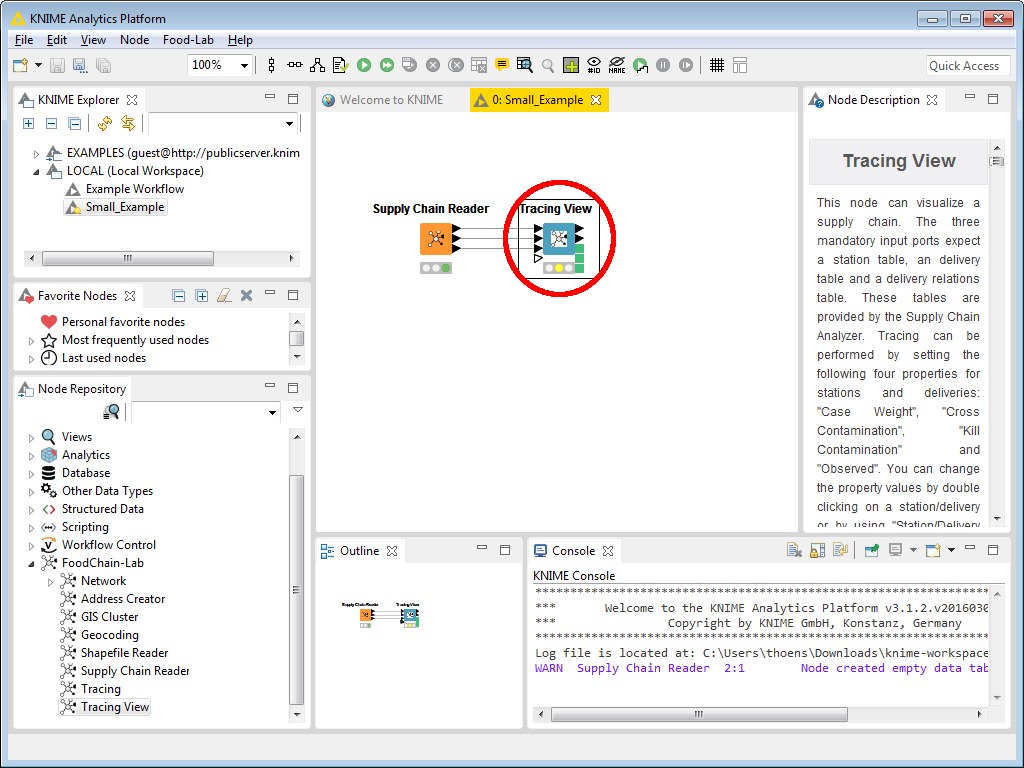
\includegraphics[height=0.6\textheight]{1.png}
	\end{center}
	\begin{itemize}
		\item Import the Small Example Workflow from \textcolor{blue}{\underline{\href{https://github.com/SiLeBAT/BfROpenLabResources/raw/master/GitHubPages/workflows/Small\_Example.zip}{``Small\_Example.zip''}}}.
		\item Open the \textbf{Tracing View} by double-clicking on it.
	\end{itemize}
\end{frame}

\section{2}
\begin{frame}
	\begin{center}
  		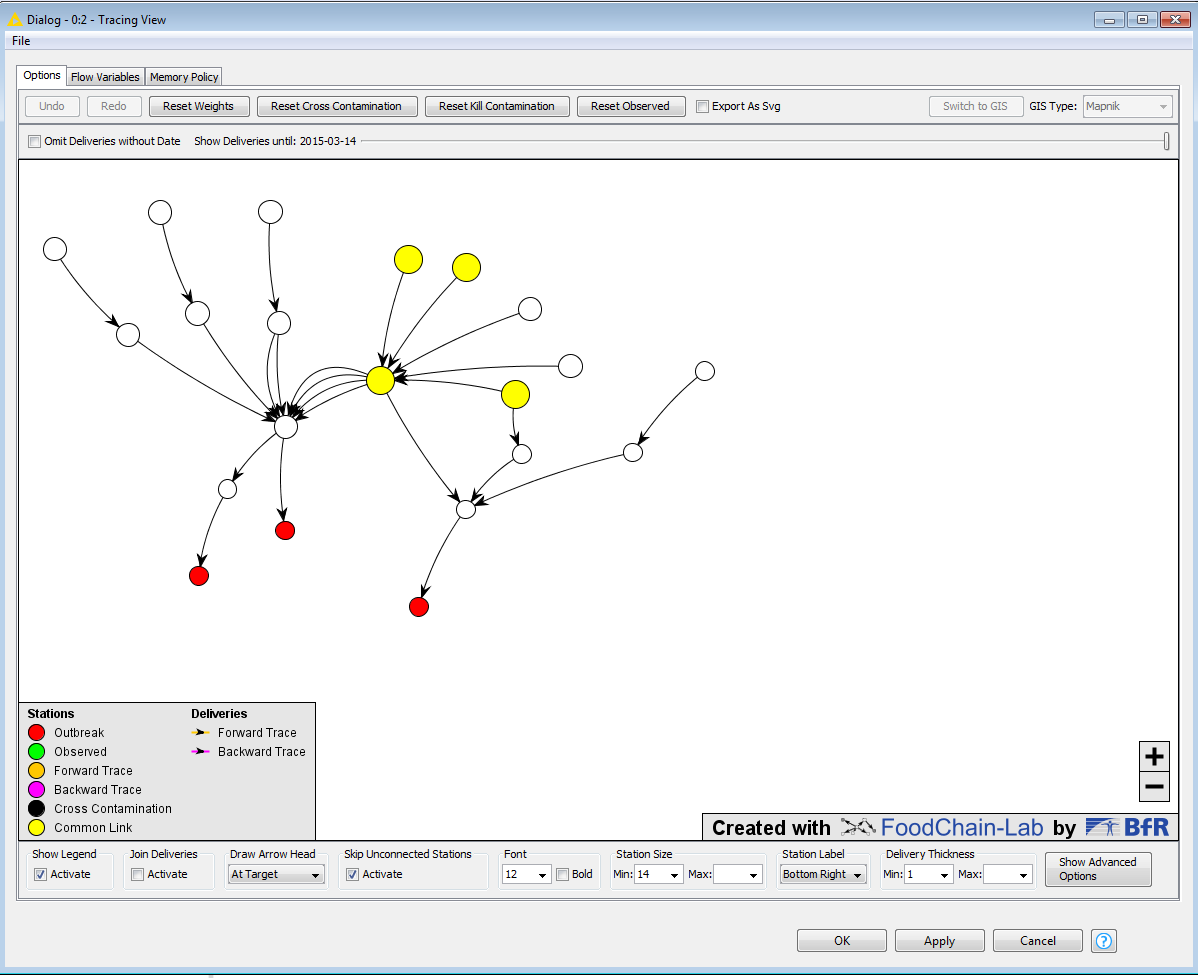
\includegraphics[height=0.6\textheight]{2.png}
	\end{center}
	\begin{itemize}
		\item Here you can see a small delivery graph with three outbreak locations (red stations) in the lower part.
	\end{itemize}
\end{frame}

\section{3}
\begin{frame}
	\begin{center}
  		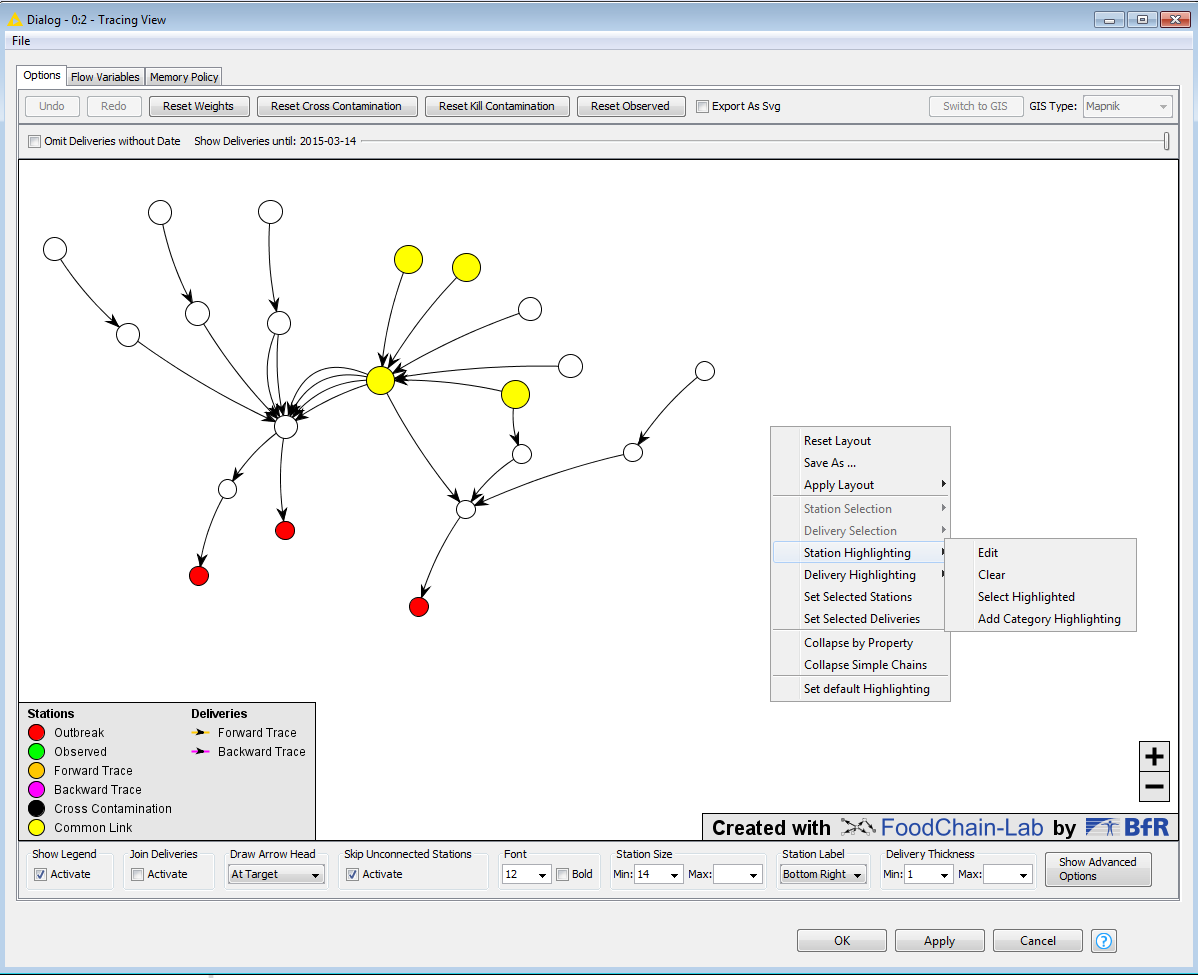
\includegraphics[height=0.6\textheight]{3.png}
	\end{center}
	\begin{itemize}
		\item Let's now change the color of the outbreak stations.
		\item Right click in the graph and select ``Station Highlighting'' and ``Edit''.
	\end{itemize}
\end{frame}

\section{4}
\begin{frame}
	\begin{center}
  		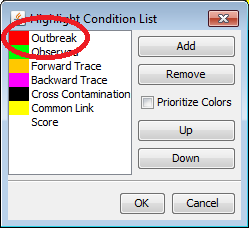
\includegraphics[scale=0.6]{4.png}
	\end{center}
	\begin{itemize}
		\item A dialog with all defined highlighting conditions will pop up.
		\item Double click on ``Outbreak'' to edit it.
	\end{itemize}
\end{frame}

\section{5}
\begin{frame}
	\begin{center}
  		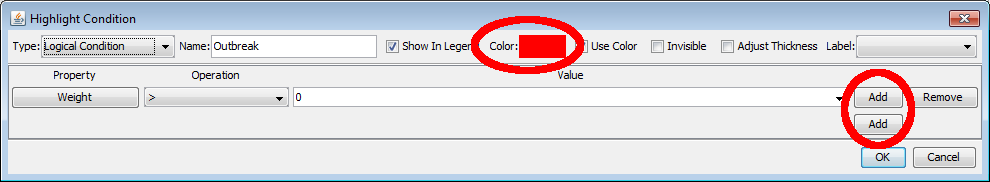
\includegraphics[scale=0.3]{5.png}
	\end{center}
	\begin{itemize}
		\item A new dialog for editing the outbreak condition will pop up.
		\item In this dialog you can also change to which stations the highlighting should be applied.
		\item Currently, all stations with "Weight" $>$ 0 are in focus. You can add other expressions by pressing the ``Add'' button on the right. These expressions can be combined via ``And'' or ``Or''.
		\item To edit the color click on the red square next to ``Color''.
	\end{itemize}
\end{frame}

\section{6}
\begin{frame}
	\begin{center}
  		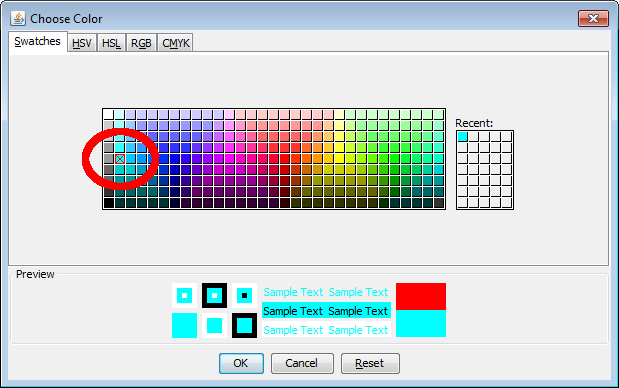
\includegraphics[height=0.6\textheight]{6.png}
	\end{center}
	\begin{itemize}
		\item In the color chooser dialog select turquoise and click ``OK''.
	\end{itemize}
\end{frame}

\section{7}
\begin{frame}
	\begin{center}
  		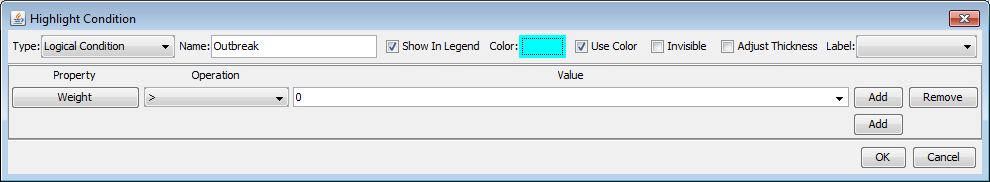
\includegraphics[width=0.9\textwidth]{7.png}
	\end{center}
	\begin{itemize}
		\item The square next to ``Color'' should be turquoise now.
		\item Press ``OK''.
	\end{itemize}
\end{frame}

\section{8}
\begin{frame}
	\begin{center}
  		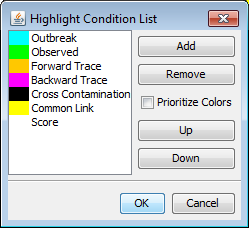
\includegraphics[scale=0.5]{8.png}
	\end{center}
	\begin{itemize}
		\item In the dialog showing all highlighting conditions press ``OK'' to apply your changes.
	\end{itemize}
\end{frame}

\section{9}
\begin{frame}
	\begin{center}
  		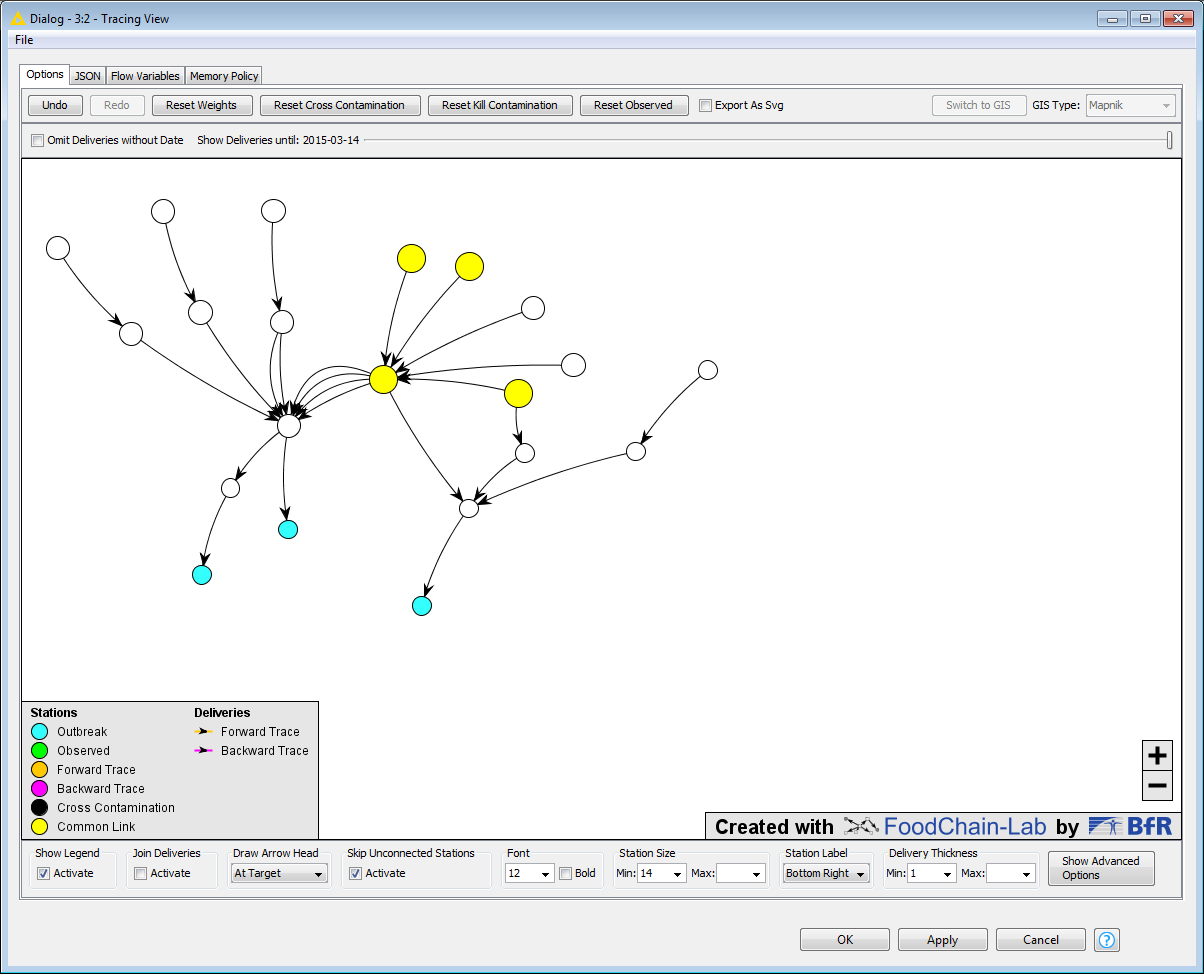
\includegraphics[height=0.6\textheight]{9.png}
	\end{center}
	\begin{itemize}
		\item The outbreak stations in the delivery graph should now be turquoise.
	\end{itemize}
\end{frame}

\section{10}
\begin{frame}
	\begin{center}
  		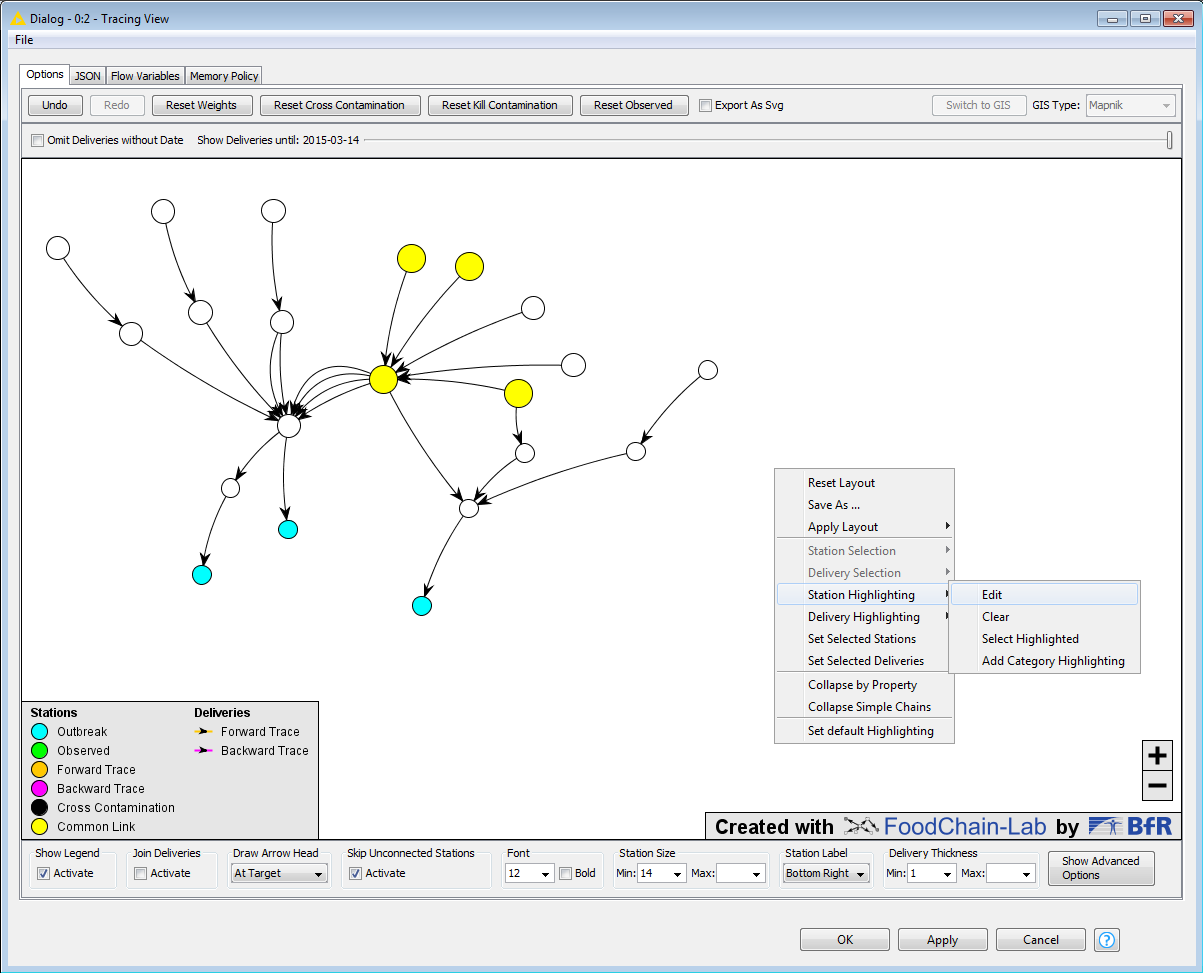
\includegraphics[height=0.6\textheight]{10.png}
	\end{center}
	\begin{itemize}
		\item Now we want to add labels to all stations in the graph.
		\item Right click in the graph and select ``Station Highlighting'' and ``Edit''.
	\end{itemize}
\end{frame}

\section{11}
\begin{frame}
	\begin{center}
  		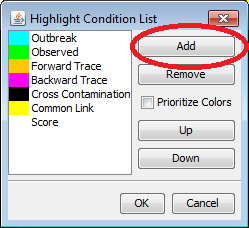
\includegraphics[scale=0.6]{11.png}
	\end{center}
	\begin{itemize}
		\item We add the labeling as a new highlight condition.
		\item Press ``Add'' to add a new condition.
	\end{itemize}
\end{frame}

\section{12}
\begin{frame}
	\begin{center}
  		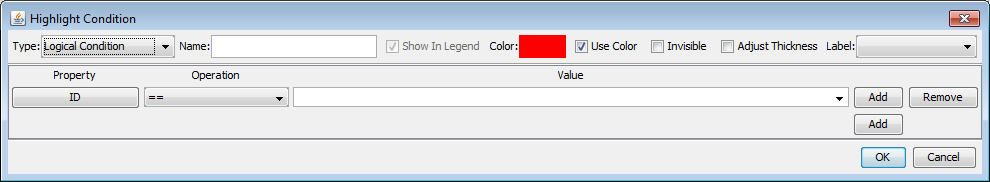
\includegraphics[width=0.9\textwidth]{12.png}
	\end{center}
	\begin{itemize}
		\item Add dialog will show up where you can configure the desired highlight condition.
	\end{itemize}
\end{frame}

\section{13}
\begin{frame}
	\begin{center}
  		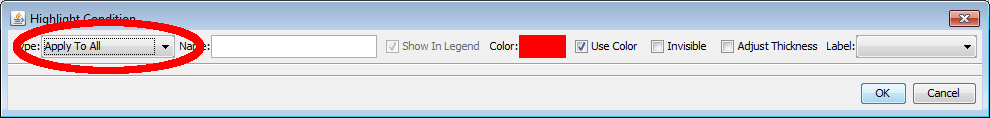
\includegraphics[width=0.9\textwidth]{13.png}
	\end{center}
	\begin{itemize}
		\item Since we want to use labels for all stations, select the type "Apply To All".
	\end{itemize}
\end{frame}

\section{14}
\begin{frame}
	\begin{center}
  		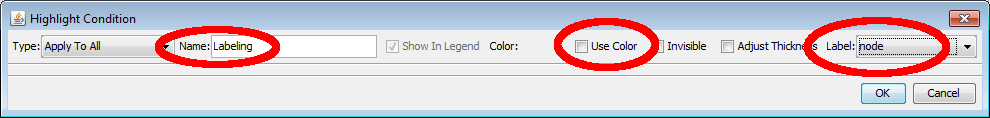
\includegraphics[width=0.9\textwidth]{14.png}
	\end{center}
	\begin{itemize}
		\item At ``Name'' you can give the highlight condition a name, for example ``Labeling'' (just for documentation).
		\item Uncheck ``Use Color'', since we just want to create labels without coloring.
		\item Set the ``Label'' to ``node''.  This option contains the station names.
		\item Click ``OK'' to create the highlight condition.
	\end{itemize}
\end{frame}

\section{15}
\begin{frame}
	\begin{center}
  		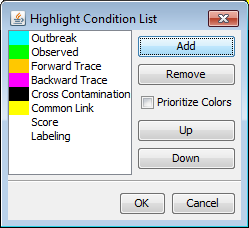
\includegraphics[scale=0.6]{15.png}
	\end{center}
	\begin{itemize}
		\item In the dialog with all highlight conditions you should now see a new condition ``Labeling''.
		\item Click ``OK'' to apply the changes.
	\end{itemize}
\end{frame}

\section{16}
\begin{frame}
	\begin{center}
  		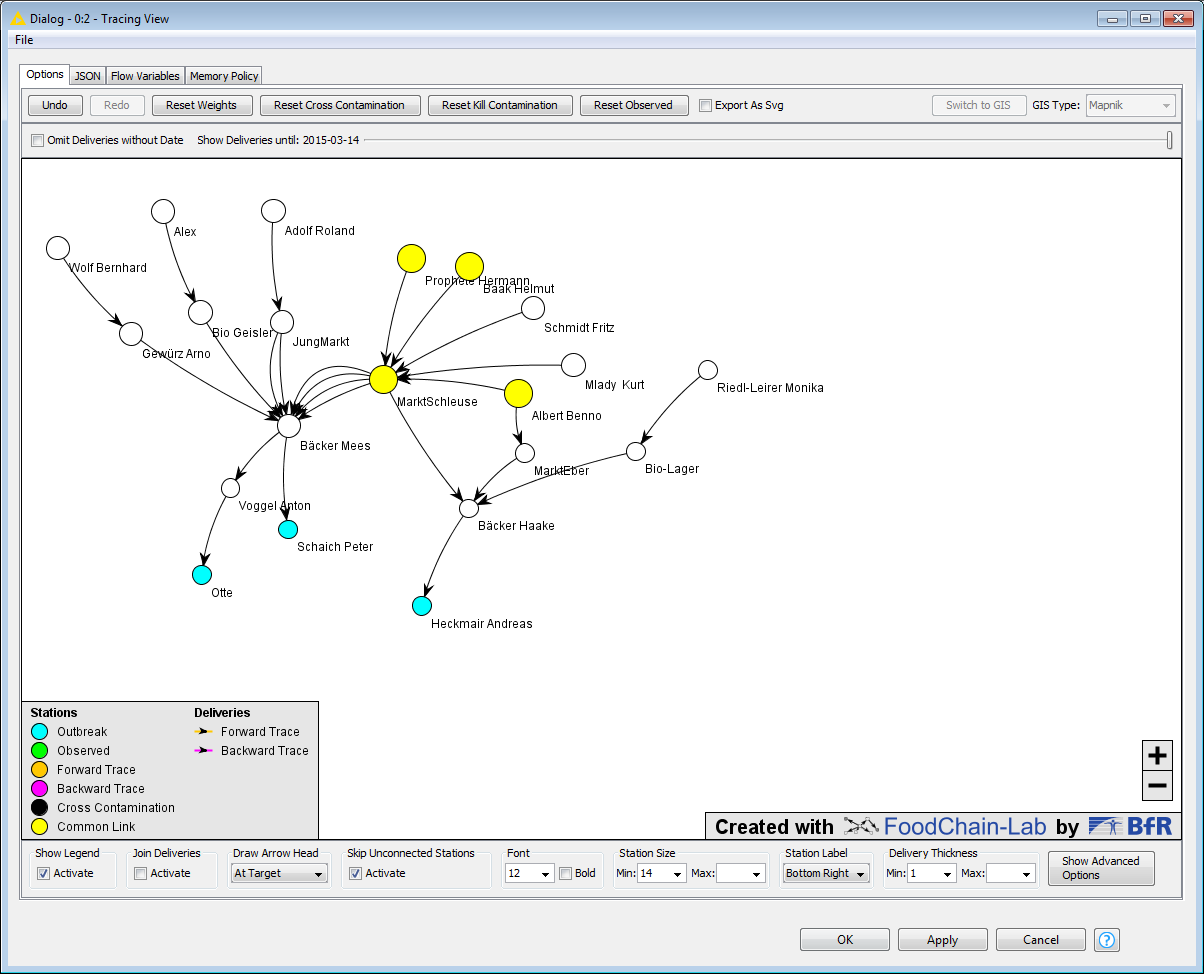
\includegraphics[height=0.6\textheight]{16.png}
	\end{center}
	\begin{itemize}
		\item In the delivery graph there is now a label next to each station. It is the station name. In the same way you could also display the tracing score, the type of business or other station data.
	\end{itemize}
\end{frame}

\section{17}
\begin{frame}
	\begin{center}
  		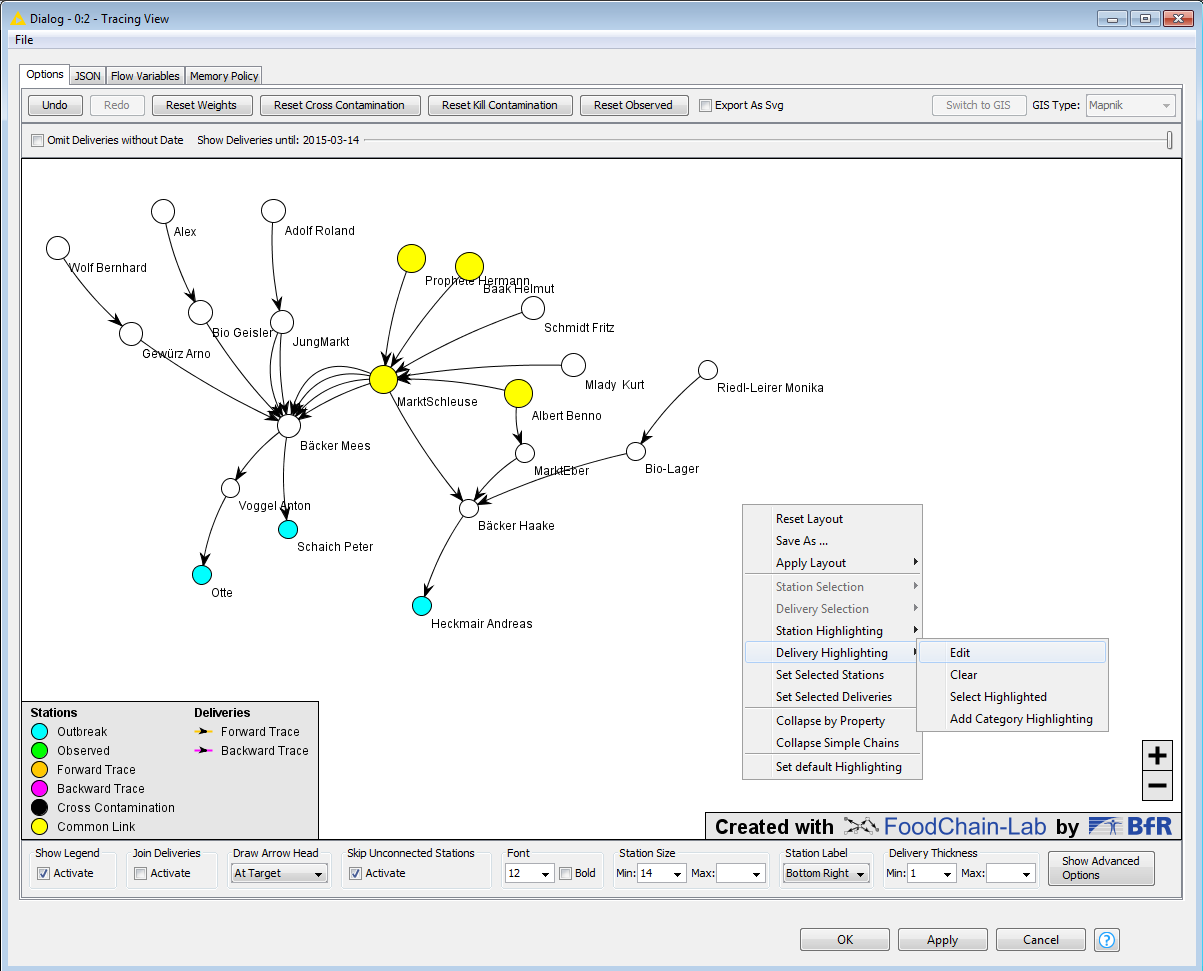
\includegraphics[height=0.6\textheight]{17.png}
	\end{center}
	\begin{itemize}
		\item FoodChain-Lab also allows to color or label deliveries the same way.
		\item To open the dialog for editing delivery highlight conditions right click in the graph, select ``Delivery Highlighting'' and ``Edit''. Then proceed in the same way as you have just done with the stations.
	\end{itemize}
\end{frame}

\end{document}
